%This file was automatically generated by [prove].

\title{Graph}
\documentclass[landscape, 11pt]{article}

\usepackage{tikz}
\usetikzlibrary{calc}
\usetikzlibrary{positioning}
\usetikzlibrary{arrows.meta}

\usepackage[margin=0pt, hoffset=0pt, voffset=0pt, top=20pt,bottom=20pt]{geometry}

\usepackage{color}
\definecolor{inactive}{rgb}{0.9, 0.9, 0.9}
\definecolor{darkmagenta}{rgb}{0.55, 0.0, 0.55}
\definecolor{darkorange}{rgb}{1.0, 0.55, 0.0}
\definecolor{darkpastelgreen}{rgb}{0.01, 0.75, 0.24}
\definecolor{oucrimsonred}{rgb}{0.6, 0.0, 0.0}
\definecolor{darkpowderblue}{rgb}{0.0, 0.2, 0.6}
\definecolor{mediumspringgreen}{rgb}{0.0, 0.98, 0.6}
\definecolor{deepskyblue}{rgb}{0.0, 0.75, 1.0}
\definecolor{brightpink}{rgb}{1.0, 0.0, 0.5}

\usepackage{calc}
\usepackage{subcaption}
\newsavebox\tlegend
\newlength\tlegendheight
\newsavebox\tgraph

\usepackage{listings}
\newlength\tgraphheight

\pagenumbering{gobble}


\begin{document}

%Legend
\sbox{\tlegend}{
\resizebox{0.9\hsize}{!}{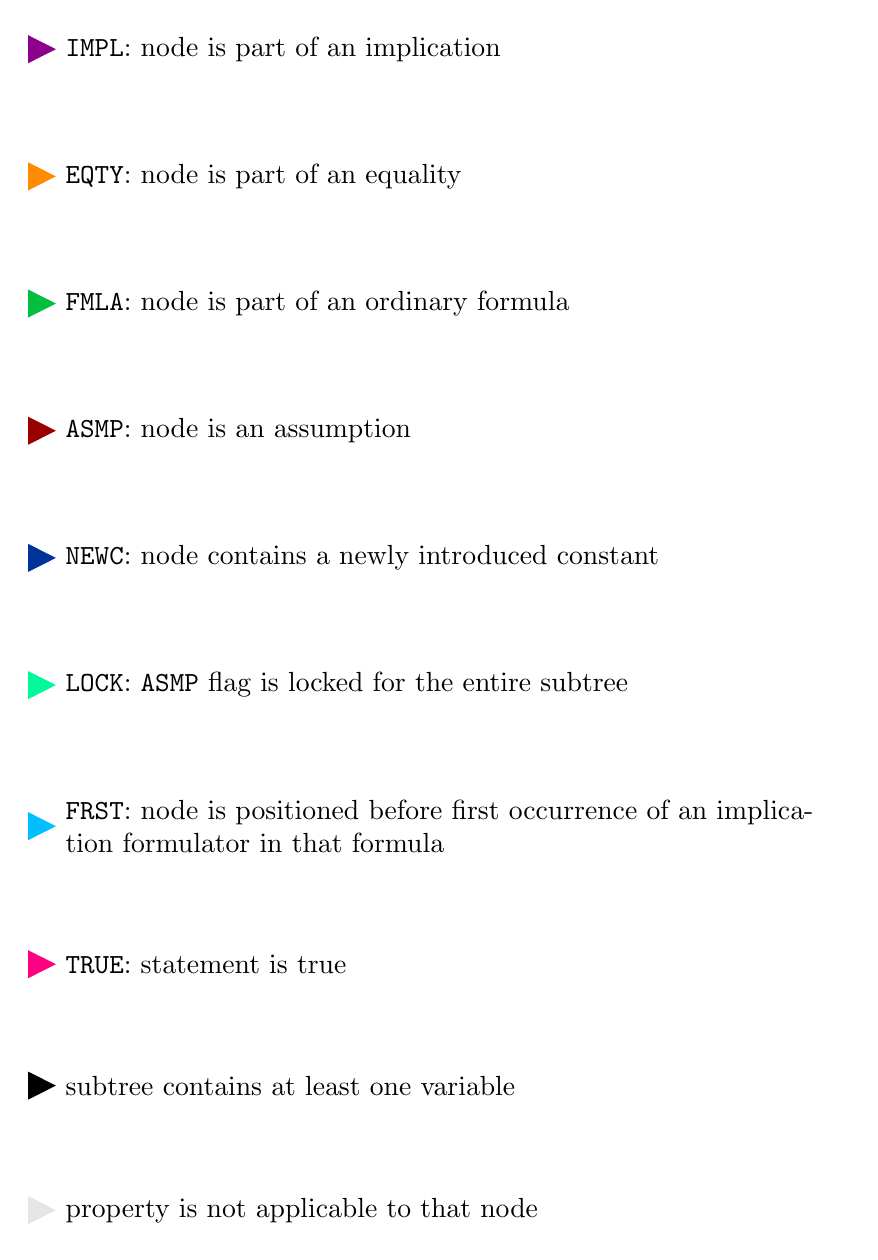
\begin{tikzpicture}[node distance = 1pt, auto]
\node[text width = 280pt, align = left, ] (IMPL) at (0pt,0pt) {\texttt{IMPL}: node is part of an implication};
\node[text width = 280pt, align = left, below = 30pt of IMPL] (EQTY){\texttt{EQTY}: node is part of an equality};
\node[text width = 280pt, align = left, below = 30pt of EQTY] (FMLA){\texttt{FMLA}: node is part of an ordinary formula};
\node[text width = 280pt, align = left, below = 30pt of FMLA] (ASMP){\texttt{ASMP}: node is an assumption};
\node[text width = 280pt, align = left, below = 30pt of ASMP] (NEWC){\texttt{NEWC}: node contains a newly introduced constant};
\node[text width = 280pt, align = left, below = 30pt of NEWC] (LOCK){\texttt{LOCK}: \texttt{ASMP} flag is locked for the entire subtree};
\node[text width = 280pt, align = left, below = 30pt of LOCK] (FRST){\texttt{FRST}: node is positioned before first occurrence of an implication formulator in that formula};
\node[text width = 280pt, align = left, below = 30pt of FRST] (TRUE){\texttt{TRUE}: statement is true};
\node[text width = 280pt, align = left, below = 30pt of TRUE] (VAR){subtree contains at least one variable};
\node[text width = 280pt, align = left, below = 30pt of VAR] (INACT){property is not applicable to that node};
\draw[-{Triangle[length=10pt,width=10pt]}, color=darkmagenta] ([xshift=-10pt] IMPL.west)to (IMPL.west);
\draw[-{Triangle[length=10pt,width=10pt]}, color=darkorange] ([xshift=-10pt] EQTY.west)to (EQTY.west);
\draw[-{Triangle[length=10pt,width=10pt]}, color=darkpastelgreen] ([xshift=-10pt] FMLA.west)to (FMLA.west);
\draw[-{Triangle[length=10pt,width=10pt]}, color=oucrimsonred] ([xshift=-10pt] ASMP.west)to (ASMP.west);
\draw[-{Triangle[length=10pt,width=10pt]}, color=darkpowderblue] ([xshift=-10pt] NEWC.west)to (NEWC.west);
\draw[-{Triangle[length=10pt,width=10pt]}, color=mediumspringgreen] ([xshift=-10pt] LOCK.west)to (LOCK.west);
\draw[-{Triangle[length=10pt,width=10pt]}, color=deepskyblue] ([xshift=-10pt] FRST.west)to (FRST.west);
\draw[-{Triangle[length=10pt,width=10pt]}, color=brightpink] ([xshift=-10pt] TRUE.west)to (TRUE.west);
\draw[-{Triangle[length=10pt,width=10pt]}, color=black] ([xshift=-10pt] VAR.west)to (VAR.west);
\draw[-{Triangle[length=10pt,width=10pt]}, color=inactive] ([xshift=-10pt] INACT.west)to (INACT.west);
\end{tikzpicture} } }

\begin{figure}[h!]\centering
\usebox{\tlegend}\end{figure}

\settototalheight\tlegendheight{\usebox{\tlegend}}
\addtolength{\tlegendheight}{50pt}
\pdfpageheight=\the\tlegendheight
\end{document}